\chapter{Background: HTTP Cookies}

Browser cookies are small bits of information sent to a client when they visit a website for the first time.
This cookie is usually saved by the user's browser for some defined period of time before it expires.
It is then sent to the website as part of the HTTP request when they revisit the site.
Using this system, the website can identify the user upon their return.

\begin{figure}[h]
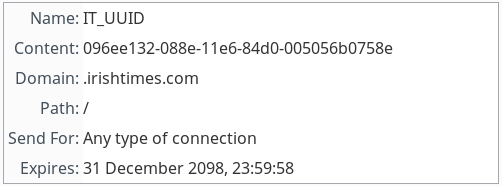
\includegraphics[scale=0.8]{cookie-example}
\centering
\caption{Example of a browser cookie}
\end{figure}

When cookies were first created, they were primarily used for remembering stateful information such as the contents of the user's shopping cart on eCommerce websites, or for recording the user's browsing activity such as whether or not they're logged in \citep{cookiesbackground}.
They're also used to allow the website to autofill previously filled in form information.
Cookies were created for this purpose because HTTP is a stateless protocol, meaning that the web servers are not required to save status information about every user on the site while they are visiting.
If the sites do want to retain information about the visitors, using browser cookies is the most common way maintaining state.

It has become standard practice for many websites to use cookies (primarily third party cookies) to track users' browsing habits and interests.
As users become more privacy aware and browser developers become more involved in protecting their users' privacy, these browser cookies are being disabled or cleared more often than before.
As the number of users allowing cookies decreases, the effectiveness of the browser cookie decreases from the advertiser's point of view, as they can not track their users over a long period of time before they have to issue them a new cookie and start over from scratch.
This is especially true for third party cookies which are likely used across a large number of websites.

\begin{figure}[h]
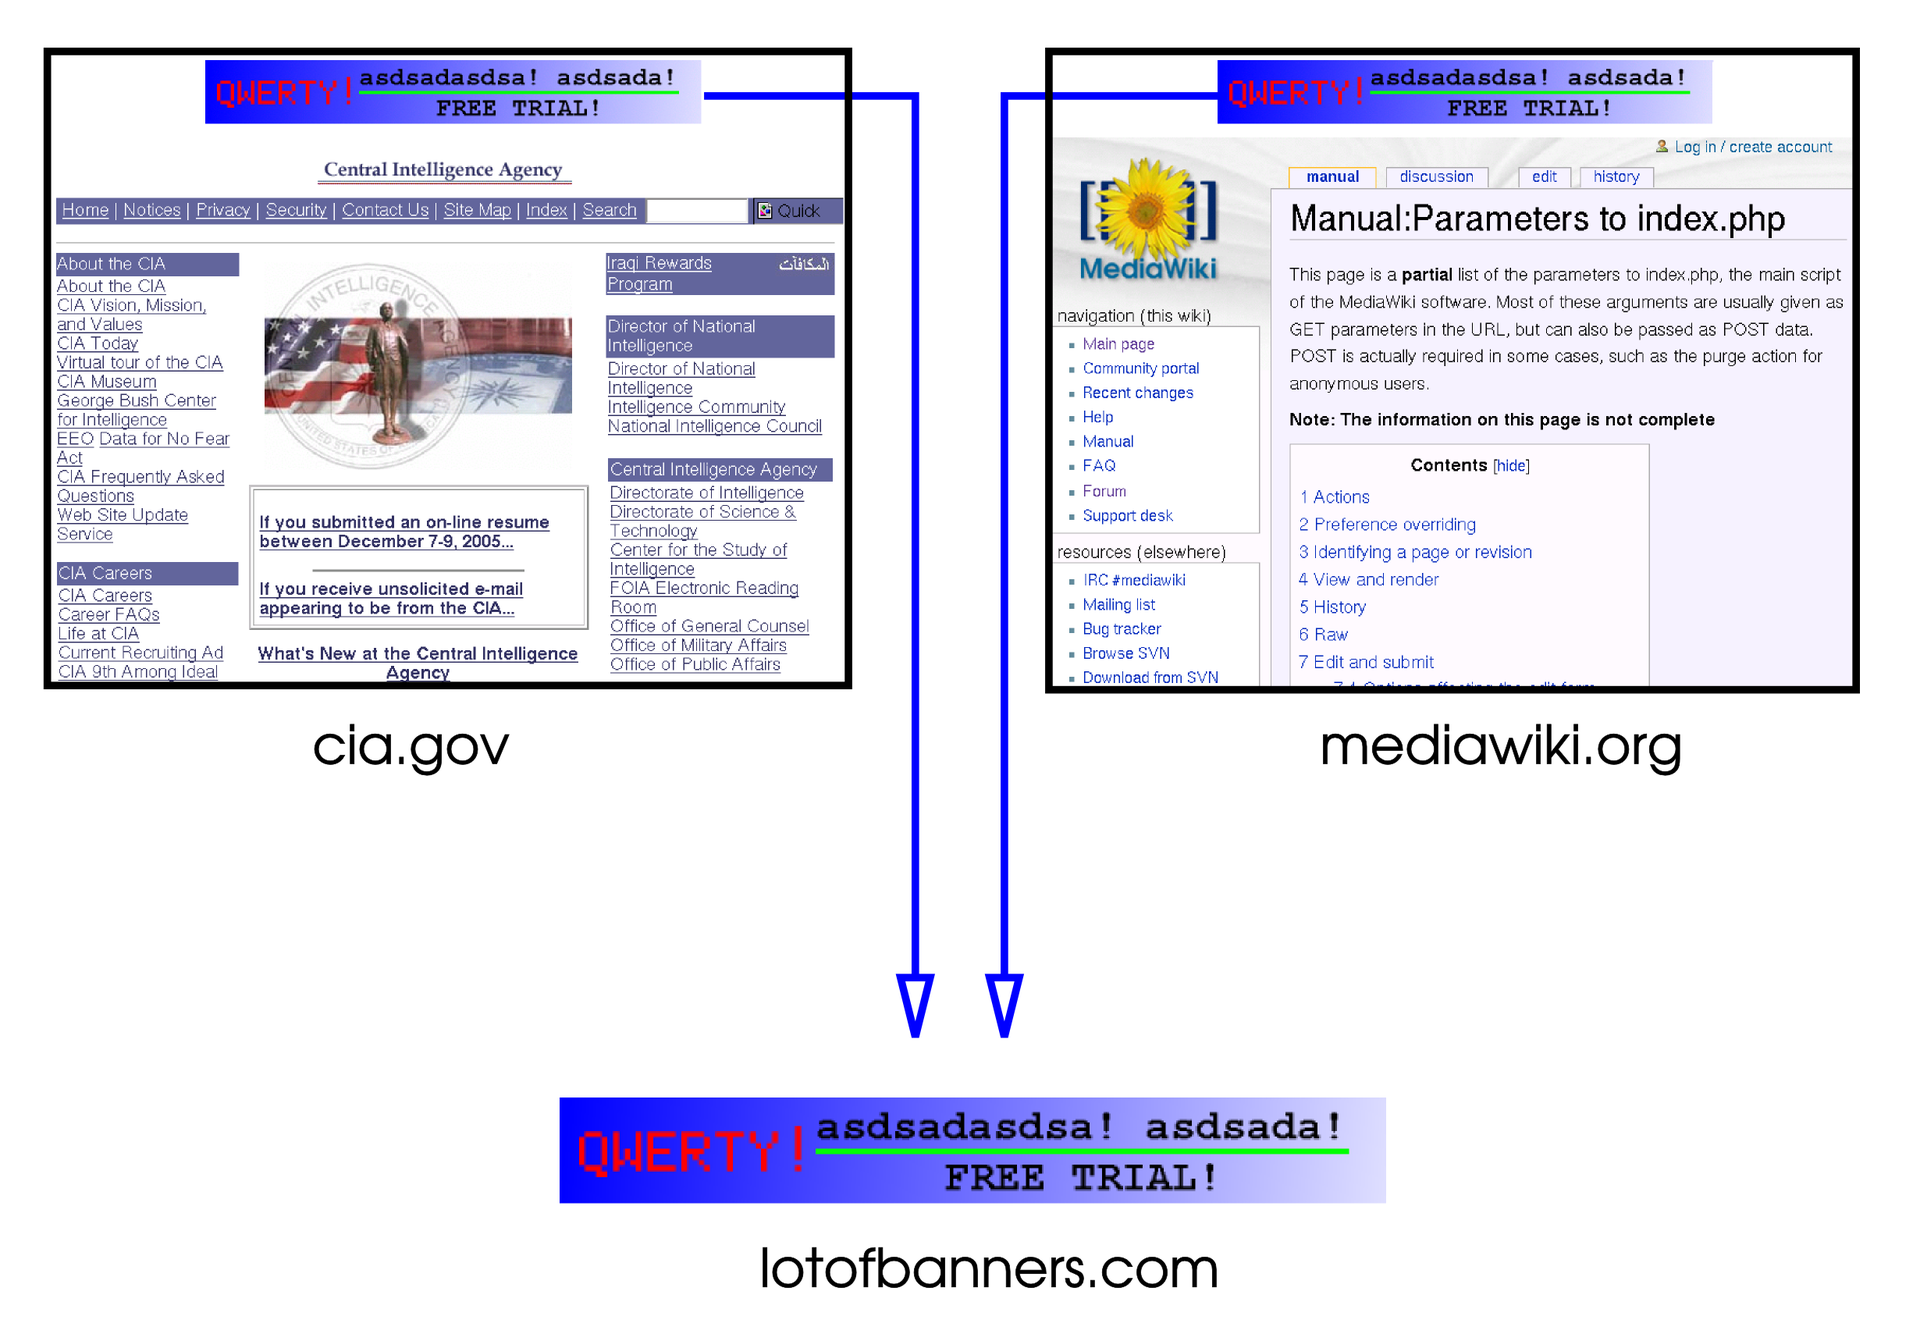
\includegraphics[scale=0.18]{third-party-cookie}
\centering
\caption{Example of a third party cookie
Here, an advertising company has a banner in two separate websites, allowing them to track the user across the two sites.}
\end{figure}

The decrease in the effectiveness of the browser cookie is what has driven some companies to find new techniques to identify and track their userbase.
They sought a more persistent alternative to a browser cookie which the user could not clear or disable.
This led to the research and use of browser fingerprinting.

